\documentclass[11pt,a4paper]{article}
\usepackage[utf8]{inputenc}
\usepackage[T1]{fontenc}
\usepackage{amsmath,amsfonts,amssymb}

\usepackage{apacite}
\usepackage{natbib}
\usepackage{graphicx}
\usepackage{booktabs}
\usepackage{threeparttable}
\usepackage{array}
\usepackage{url}
\usepackage{hyperref}
\usepackage[margin=2.5cm]{geometry}
\usepackage{setspace}
\usepackage{comment}
\usepackage{outlines}
\onehalfspacing
%\doublespacing

\newcommand{\tablepath}{papers/econometrics/table}
\newcommand{\figurepath}{papers/econometrics/figure}

\newcommand{\Var}{\text{Var}}
\newcommand{\Cov}{\text{Cov}}

\DeclareMathOperator*{\plim}{plim}

% Define \sym command for significance stars from esttab
\newcommand{\sym}[1]{{#1}}

\title{CEO Replacements and Firm Growth: Correcting for Small-Sample Bias in Fixed-Effect Estimates\thanks{We thank Ot\'{a}vio Bartalotti and St\'ephane Bonhomme for helpful discussions and comments.  We thank the excellent assistance provided by Gergely Attila Kiss. The paper benefited from presentations at the Universit\'a della Svizzera Italiana and Corvinus Empirical Seminar. Project No. 144193 has been implemented with the support provided by the Ministry of Culture and Innovation of Hungary from the National Research, Development and Innovation Fund, financed under the KKP\_22 funding scheme. This project was funded by the European Research Council (ERC Advanced Grant agreement number 101097789). Telegdy received support from the Hungarian Scientific Research Fund – OTKA, contract number 143346. The views expressed in this research are those of the authors and do not necessarily reflect the official view of the European Union or the European Research Council or the National Research, Development and Innovation Fund.}}

\author{Miklós Koren\thanks{Central European University, ELTE Centre for Economic and Regional Studies, CEPR and CESifo. E-mail: korenm@ceu.edu} \\
        Krisztina Orbán\thanks{Monash University. E-mail: krisztina.orban@monash.edu} \\
        Álmos Telegdy\thanks{Corvinus University of Budapest. E-mail: almos.telegdy@uni-corvinus.hu}}

\date{August 2026}

\begin{document}

\maketitle
\thispagestyle{empty}

\begin{abstract}
\noindent We develop a placebo-controlled method to correct small-sample bias in firm–CEO two way fixed-effects estimates. The approach exploits within-firm CEO replacements and measures changes in CEO quality from differences in firm performance across adjacent CEO spells. Placebo transitions are assigned to matched firms without CEO changes, allowing us to identify and remove bias in second moments and event-study estimates. Monte Carlo simulations show that the method accurately recovers true variances, covariances, and dynamic effects in short panels. Applying the method to the universe of Hungarian firms, we find that conventional estimators substantially overstate the importance of CEOs and generate spurious pre-trends before CEO transitions.
\end{abstract}

\textbf{Keywords:} CEO value, CEO-Firm Fixed Effects, Bias Correction, Hungary, SMEs

\textbf{JEL Classification:} C23, D24, G34

\clearpage
\setcounter{page}{1}

%%%%%%%%%%%%%%%%%%%%%%
\section{Introduction}
%%%%%%%%%%%%%%%%%%%%%%

%TWFE literature on managers
The role of managers in shaping firm outcomes has attracted substantial attention in economics, finance, and management. Because researchers rarely observe the managerial traits relevant for firm behavior, the dominant empirical approach studies the role of managers by capturing managerial heterogeneity through firm and manager fixed effects. These studies find that managers account for a substantial share of variation in firm outcomes.

A central challenge of the two-way fixed effects estimation is that managerial spells in firms are usually short. As a consequence, estimated manager effects are noisy, and any statistic involving second moments are subject to limited mobility bias even if many CEO transitions are observed \citep{kline2024firm}. A growing methodological literature has therefore focused on correcting biases in second moments of estimated fixed effects. These include parametric corrections for estimation error \citep{andrews2008high, gaure2014correlation}, leave-one-out estimators \citep{kline2020leave}, and approaches based on grouping observations to reduce dimensionality \citep{Bonhomme2019-xi,bonhomme2023much}. While these contributions have substantially improved inference, they rely on settings where managerial mobility across firms is sufficiently rich to identify managerial heterogeneity from observed movements across organizations.

%Limitations of the literature
Existing evidence on managerial effects typically concerns large, often publicly listed corporations, where managers switch firms and where rich information on executives is available (as we detail at the end of this section).\footnote{Even among large firms, external CEO appointments remain the exception rather than the rule. Among the listed companies of the US, 72\% of CEO hires are internal promotions and over 80\% are current or former employees or board members \citep{cziraki2022market}.} Much less is known about managerial effects among small and medium-sized enterprises (SMEs), despite that they account for roughly two-thirds of employment in advanced economies and an even larger fraction in developing countries \citep{MadgavkarEtAl2024_MSMEs}. In these firms managers typically spend most or all of their careers at a single firm, and little information on firm outcomes is available beyond standard accounting records. As a result, the approach used in the literature would exclude most firms and managers from analysis, leaving open the question of how important managers are in the broader population of firms. Moreover, the estimation sample is further reduced because the standard two-way fixed effects estimation can only be applied to the connected component of the data. These requirements reduce the share of firms which can be used in the analysis making estimates imprecise due to small sample problems. The small sample also calls into question the external validity of the results if SMEs which switch CEOs are different from the bulk of firms which do not.\footnote{\cite{cziraki2022market} shows that among the US listed companies, external hiring depends of firm characteristics.}

%summary in one para
This paper makes three contributions. First, we develop an estimator that recovers unbiased second moments of CEO-spell effects under mild identification assumptions and corrects the bias in variance decompositions and event-study coefficients. Second, we construct a new dataset linking CEOs to the universe of almost half million Hungarian firms for the period of 1992 -- 2023. Third, we use the new dataset and methodology to quantify the importance of managerial heterogeneity in SMEs, showing that conventional estimators substantially overstate the explanatory power of CEO changes and generate spurious dynamic patterns around CEO transitions. 

%starting point
The starting point of our estimation is a standard two-way fixed effects model in which the dependent variable is a measure of firm performance (e.g., revenue), while firm and CEO effects capture persistent heterogeneity across firms and managers. Specifically, firm performance is modeled as the sum of a firm fixed effect, a CEO-spell fixed effect, and a transitory error term.

%use only within firm ceo changes
Because CEO mobility across firms is relatively rare among SMEs, we use within-firm CEO replacements for identification. Instead of using separate CEO fixed effects, we transform the two-way fixed-effects model into first differences, which removes the firm fixed effect from the specification and estimate the variation of firm outcomes around the CEO change. The key advantage of this approach is that it can be applied to the full set of firms experiencing a CEO transition, substantially enhancing the power of the analysis and the external validity of the estimates. Moreover, the method does not require restricting the sample to the largest connected component of the CEO–firm network, since we do not rank CEOs in the sample. Our aim is more modest: we only aspire to identify how the change of CEOs within a firm explains changes in firm attributes.

%description of the method
To correct the small-sample bias inherent in estimated CEO fixed effects, we introduce a \textit{placebo-controlled debiasing} method. To each firm with a CEO change, we assign a matched control firm that does not change its CEO during the same period. We then assign the control firm a placebo CEO transition in the same year as the treated firm, replicating the treated firm's spell structure. Because no actual CEO change occurs in the placebo firm, any estimated variance, covariance, or event-study ``effect'' measured around the placebo transition reflects only estimation noise arising from short CEO spells and persistent firm-level shocks. Thus, changes around the placebo CEO replacement can be used to purge the estimated effect of CEO change from the idiosyncratic noise arising from the short time series of CEO spell.\footnote{Using firms which do not change CEOs to control for noise in the data is in the spirit of \cite{fitza2014use} and \cite{jarosiewicz2023revisiting}.}

Our estimation uses two identifying assumptions. The first is the standard \textit{exogeneity assumption} and states that changes in CEO-spell effects are uncorrelated with firm-level shocks. Under this assumption, the estimated change in the CEO effect is an unbiased measure of the true change in CEO quality. We call the second identifying assumption the \textit{proportional autocovariance assumption}, which states that the variance-covariance matrix of shocks is identical in the treated and placebo samples up to a scalar multiplier. This assumption requires the temporal correlation structure of idiosyncratic firm-level shocks to be the same across the treated and placebo groups. At the same time, it allows firms which replace their CEO to experience larger or smaller idiosyncratic shocks than firms with stable CEOs. Conceptually, the proportional autocovariance assumption resembles the parallel trends assumption in difference-in-differences designs. Our method can be viewed as difference-in-differences for second moments: we difference out the bias by comparing treated and control firms' variances and covariances.

Under the two assumptions, the placebo sample reproduces the same small-sample bias present in the treated sample. Subtracting the placebo moments from the corresponding moments based on the treated firms yields unbiased estimates of CEO-related variance, covariance, and dynamic treatment effects.

%what we use the method for
We construct two statistics, which contain the second moments of the data and thus are contaminated by the small sample bias. The first is the $R^2$ of the estimation, which measures the share of the variance of the firm variable attributable to CEO change. The second is a full set of event-time coefficients, which shows both the trend in the dependent variable pre-transition and its post-transition dynamics. These features are particularly important because pre-trends are commonly used to assess the validity of the identification strategy, while the shape of the post-transition response reveals how quickly CEO effects materialize and whether they persist over time. 

%MC
CHANGE We test the validity of the placebo-controlled debasing in Monte Carlo experiments designed to mimic the characteristics of firm-level panels with CEO transitions. The simulations generate firms with two CEO spells and outcomes determined by a CEO effect and an idiosyncratic shock process. We consider a range of empirically relevant environments, including short CEO tenures (the baseline scenario), persistent shocks, excess variance in treated firms, all complications at the same time, long panels and a pre-trend (to check how the method performs when some of the identifying assumptions are not satisfied). The experiments show that conventional estimators substantially overstate the variance of CEO effects and can generate spurious pre-trends and distorted post-transition dynamics even when the identifying assumptions hold. In contrast, the placebo-controlled estimator consistently recovers the true variances, covariances, and event-study coefficients across all scenarios. These results demonstrate that the method is robust to all the complications we inserted in the data.

%application
We apply the placebo-controlled debiasing method to the universe of Hungarian firms between 1992 and 2023, leveraging administrative data that link CEOs to firm balance sheets and income statements. The data cover the population of SMEs (471,000 firms and over 2.5 million firm-years), 475,000 distinct CEOs and about 266,000 within firm CEO transitions.\footnote{Perhaps the best alternative of our method is the leave-one-out method \citep{kline2020leave}. This method is based on the sample of firms which have a CEO transition where both CEOs also served in another firm. In addition, this method can be performed only on the connected component of the data. The final sample is XX firms, only XX\% of the data.}

We estimate the variation of several firm attributes around CEO transitions:  output, inputs (labor and capital), and productivity (return on assets and labor productivity. The empirical results show that conventional estimators substantially overstate the importance of CEOs. The $R^2$ of conventional estimates is 0.65-0.75, whereas the debiased estimates imply $R^2$s between 0.19-0.29. The explanatory power of the estimation is larger when the incumbent and the new CEO differ along some dimension (founder–nonfounder, female–male, age), or when one CEO cleanly replaces another, rather than cases where one CEO remains permanently with the firm while a second CEO leaves or joins. We also find that event-study estimates based on conventional methods display pronounced pre-trends that disappear after debiasing, indicating that they are artifacts of small-sample bias rather than evidence against the identification strategy. 

%litrev
\paragraph{Literature.} Our work connects primarily to the literature using firm and manager fixed effects to estimate the CEO influence on firm policy. \cite{Bertrand2003-io} was the first to use two-way fixed effects to study the importance of managers, and showed that CEOs influence investment, growth, productivity and other firm outcomes. Researchers connected managerial fixed effects with profitability \citep{mackey2008effect}, risk taking \cite{schoar2024effect}, and employee quality \citep{lazear2015value} (this paper used manager and worker fixed effects). Papers established that CEO effects increase over time \citep{quigley2015has} and are correlated with nationwide institutions, such as the origin of the legal system, labor market flexibility, and ownership structure \citep{crossland2011differences}. These studies use data from listed companies. \cite{quigley2022ceo} uses data of large listed and private companies, and finds that that CEOs affect private firms to a larger extent. One exception in terms of firm size is \cite{baltrunaite2023managerial}, who use the universe of Italian limited liability companies over 20 employees. The paper finds that managerial quality is associated with the adoption of better managerial practices.  

In contrast to these datasets, our study uses the universe of Hungarian firms (we only drop corporations with fewer than 2 employees on average). For identification, our method uses all the firms which experience a CEO change (about a quarter of million transitions) and we do not need to restrict the sample to the connected component. 

Similar methods were also applied to the public sector and also find that CEOs are important in this area as well \citep{fenizia2022managers, janke2024role}. 

Methodologically, we connect to the literature correcting the limited mobility bias in two-way fixed effects analysis. In terms of variance-covariance correction, three broad methods are proposed: assuming and estimating a parametric model for error covariance structure \citep{andrews2008high,gaure2014correlation,kline2024firm}, leave-one-out adjustments \citep{kline2020leave}, and grouping observations to reduce the number of parameters to be estimated \citep{Bonhomme2019-xi}. Parametric methods require correctly specifying and estimating complex autocorrelation patterns, while our method needs only mild identifying assumptions. The leave-one-out method is impractical in CEO markets where most managers work at only one firm and mobility is limited. Since our interest is understanding heterogeneity of CEOs and factors that correlate with this heterogeneity, keeping the original dimensionality of the data is preferable. 

The main difference between the methods described above and our is the we estimate from within firm, rather than between firm, CEO changes. Similar approach was employed \cite{fitza2014use} and \cite{jarosiewicz2023revisiting}. They state that the limited mobility bias distorts the second estimated moments of CEO fixed effects and use placebo CEO switches to correct for this bias. They do not, however, demonstrate formally under what identifying assumptions will the corrected estimate be unbiased, nor they correct for the coefficients of event time analysis. In addition, they use listed firms while we use the whole Hungarian population. 

%Finally, event studies are used to assess how outcomes evolve before and after CEO transitions to test for pre-trends and to understand post-transition dynamics \citep{schoar2024effect}.

Our paper also builds on the two-way fixed effects literature in labor economics that decomposes wages into worker and firm components (see the recent review of \citep{kline2024firm}. Unlike the labor literature, our focus is on understanding manager fixed effects rather than firm fixed effects. We include firm fixed effects in our estimation model, but remove them in the estimation step by differencing or demeaning, so we cannot comment on the correlation between firm and worker (CEO) effects, a common question in labor studies.

The paper proceeds as follows. Section \ref{sec:econometric_problem} presents the econometric problem, explains briefly the small sample bias and shows its implication on commonly used statistics. Section \ref{sec:placebo_debiasing} introduces the placebo-controlled debiasing method, which we evaluate in Section \ref{sec:MC} with Monte Carlo estimations. Section \ref{sec:application} applies the method to CEO transitions in Hungarian firms and studies the role of managerial heterogeneity in shaping firm outcomes. Section \ref{sec:concl} concludes.


%%%%%%%%%%%%%%%%%%%%%%%%%%%%%%%%%
\section{The Econometric Problem}\label{sec:econometric_problem}
%%%%%%%%%%%%%%%%%%%%%%%%%%%%%%%%%

Let $q_{it}^{k}$ denote measure $k$ of firm $i$'s performance in year
$t$. Such measures can include log
revenue, return on assets, log labor productivity and so on. For each measure
$k$, we write
\begin{equation}
q_{it}^{k}
=
\alpha_i^{k}
+
z_{is(i,t)}^{k}
+
e_{it}^{k},
\label{eq:outcome_model}
\end{equation}
where $\alpha_i^{k}$ is a firm fixed effect, $s(i,t)$ indexes the CEO
spell in place at firm $i$ in year $t$, and $z_{is(i,t)}^{k}$ is the
component of firm performance associated with that CEO spell. The spell component is constant during a CEO spell and changes when the firm replaces the CEO. The remaining variation is captured by the firm-level
shock $e_{it}^{k}$.

Let $\mathcal S_i$ denote the set of CEO spells observed at firm $i$.
We impose strict exogeneity:
\begin{equation}
E\!\left[
e_{it}^{k}
\mid
\alpha_i^{k},
\{z_{is}^{k}\}_{s\in\mathcal S_i}
\right]
=
0
\qquad
\text{for every }t.
\label{eq:strict_exogeneity}
\end{equation}
This assumption ensures that the average shock within each CEO spell is
zero in expectation. Consequently, the difference between the average
outcomes observed in two adjacent spells is an unbiased measure of the
change in the CEO-spell component.

The object $z_{is}^{k}$ is a firm-specific CEO-spell effect, rather than
a portable person effect that follows the CEO across firms. A large share of the CEOs
in our comprehensive dataset are observed at only one firm, therefore we do not use mobility
across firms to identify their effects. The spell component may capture
the CEO's skill, the match between the CEO and the firm, or other
persistent features associated with that particular CEO spell.
Throughout the paper, we refer to it as a CEO effect for
brevity, but the empirical object is the component of firm performance
associated with a CEO spell at a particular firm.

%%%%%%%%%%%%%%%%%%%%%%%%%%%%%%%%%%%%%%%%%%%%
\subsection{Changes in CEO-spell components}\label{subsec:spell_changes}
%%%%%%%%%%%%%%%%%%%%%%%%%%%%%%%%%%%%%%%%%%%%

Our interest is not in the level of the firm fixed effect, hence to remove $\alpha_i^{k}$, we difference outcomes across adjacent CEO spells within the same firm. As we are interested in changes within the firm, we do not need to restrict our attention only to the connected CEO-firm mobility network, and we can study all firms with a CEO replacement. For firm $i$, consider two adjacent CEO spells, $s-1$ and $s$. The
true change in the CEO-spell component measured using outcome $k$ is
\begin{equation}
\Delta z_{is}^{k}
=
z_{is}^{k}
-
z_{i,s-1}^{k}.
\label{eq:true_spell_change}
\end{equation}

We do not observe either spell component directly. Let $T_{is}$
denote the number of years in which firm $i$ is observed during CEO
spell $s$. We estimate the difference between the two spell components
using the difference between the average outcomes observed during the
two spells:
\begin{equation}
\Delta\widehat z_{is}^{k}
=
\frac{1}{T_{is}}
\sum_{t:\,s(i,t)=s}
q_{it}^{k}
-
\frac{1}{T_{i,s-1}}
\sum_{t:\,s(i,t)=s-1}
q_{it}^{k}.
\label{eq:estimated_spell_change}
\end{equation}

Substituting Equation~\eqref{eq:outcome_model} into
Equation~\eqref{eq:estimated_spell_change}, the firm fixed effect
cancels, and the estimated spell change can be written as
\begin{equation}
\Delta\widehat z_{is}^{k}
=
\Delta z_{is}^{k}
+
\frac{1}{T_{is}}
\sum_{t:\,s(i,t)=s}
e_{it}^{k}
-
\frac{1}{T_{i,s-1}}
\sum_{t:\,s(i,t)=s-1}
e_{it}^{k}.
\label{eq:spell_change_error}
\end{equation}
The last two terms constitute the estimation error in the measured
change in the CEO-spell component.

Under strict exogeneity,
\begin{equation}
E\!\left[
\Delta\widehat z_{is}^{k}
\mid
\Delta z_{is}^{k}
\right]
=
\Delta z_{is}^{k}.
\label{eq:unbiased_spell_change}
\end{equation}
Therefore, under strict exogeneity, the estimated change is unbiased, regardless of the number of observations within the two spells. If the
number of observations within both spells were large enough for the
average firm-level shocks to converge to zero, the estimated change
would also converge to the true CEO-spell change. In typical CEO-firm
panels, however, CEO spells are short. As a result, the estimated
changes can remain substantially noisy even though they are unbiased.

This is the source of the small-sample bias in statistics constructed from the estimated CEO-spell changes. Even when the number of firms and observed CEO changes is very large, each individual spell-change estimate remains noisy if the number of years observed within the two spells is small. A larger number of firms allows us to estimate moments of the distribution of the noisy spell-change estimates more precisely, but it does not eliminate the noise contained in each estimate. Consequently, even with many firms, the variance of the estimated spell changes and their covariance with estimated changes in other outcomes may differ systematically from the corresponding variance and covariance of the true spell changes.

We study how a firm outcome changes when firm $i$ moves from CEO spell
$s-1$ to $s$. Let $q_{it}^{j}$ denote outcome $j$ of firm $i$ in
year $t$. The outcome $j$ need not be the same variable as the measure
$k$ used to construct the CEO-spell change. For example, we may measure
the change in the CEO-spell component using revenue and study how
employment, capital, profitability, labor productivity, or exporter
status changes when the firm changes CEO.

Let $g_{is}$ denote the first year of CEO spell $s$ at firm $i$. For
event time $h$, define the outcome contrast
\begin{equation}
\Delta_h q_{is}^{j}
=
q_{i,g_{is}+h}^{j}
-
q_{i,g_{is}-1}^{j}.
\label{eq:outcome_contrast}
\end{equation}
Thus, the outcome in each event year is measured relative to the final
year of the preceding CEO spell. The same argument applies to more
general linear contrasts, including the difference between average
post-transition and pre-transition outcomes.


%%%%%%%%%%%%%%%%%%%%%%%%%%%%%%%%%
\subsection{Second moment biases}\label{subsec:variance_bias}
%%%%%%%%%%%%%%%%%%%%%%%%%%%%%%%%%

The short CEO spells bias both the variance $\operatorname{Var}\!\left(
\Delta\widehat z_{is}^{k} \right)$ and the covariance between $\Delta\widehat z_{is}^{k}$ and the change in the firm attribute, $\operatorname{Cov}\!\left(\Delta\widehat z_{is}^{k},\Delta_h q_{is}^{j}\right)$.
\vspace{.2cm}

\paragraph{Bias in the variance.} The noise in the estimated CEO-spell change is the difference between the average firm-level shocks in spells $s$ and $s-1$.\footnote{For formal derivations of the biases, see Appendix \ref{sec: appA}.} Let the variance
of this estimation error be
\begin{equation}
B^{k}
=
\operatorname{Var}\!\left(
\frac{1}{T_{is}}
\sum_{t:\,s(i,t)=s} e_{it}^{k}
-
\frac{1}{T_{i,s-1}}
\sum_{t:\,s(i,t)=s-1} e_{it}^{k}
\right)
\geq 0.
\label{eq:B_definition}
\end{equation}

Using the decomposition of the estimated CEO-spell change, its variance
is
\begin{align}
\operatorname{Var}\!\left(
\Delta\widehat z_{is}^{k}
\right)
={}&
\operatorname{Var}\!\left(
\Delta z_{is}^{k}
\right)
+
B^{k}
\nonumber\\
&+
2\operatorname{Cov}\!\left(
\Delta z_{is}^{k},
\frac{1}{T_{is}}
\sum_{t:\,s(i,t)=s} e_{it}^{k}
-
\frac{1}{T_{i,s-1}}
\sum_{t:\,s(i,t)=s-1} e_{it}^{k}
\right).
\label{eq:variance_decomposition}
\end{align}

Strict exogeneity implies that the final covariance is zero.
Consequently,
\begin{equation}
\operatorname{Var}\!\left(
\Delta\widehat z_{is}^{k}
\right)
=
\operatorname{Var}\!\left(
\Delta z_{is}^{k}
\right)
+
B^{k}.
\label{eq:variance_bias}
\end{equation}

The observed dispersion in estimated CEO-spell changes therefore
combines genuine heterogeneity in spell changes with dispersion
generated by firm-level shocks. A variance decomposition based directly
on $\Delta\widehat z_{is}^{k}$ will consequently overstate the variance
of the true CEO-spell changes.

The magnitude of $B^{k}$ depends on the lengths of the two spells and
on the temporal covariance structure of the firm-level shocks. Short
spells generally produce more estimation error because each spell
average is calculated from fewer observations. Correlation among shocks
within a spell affects the precision of each spell average, while
correlation between shocks in the two adjacent spells affects the
precision of their difference.

This variance distortion does not disappear as the number
of firms with CEO replacements increases. If spell lengths remain bounded, then, as the number of observed adjacent spell pairs grows,
\begin{equation}
\widehat{\operatorname{Var}}\!\left(
\Delta\widehat z_{is}^{k}
\right)
\overset{p}{\longrightarrow}
\operatorname{Var}\!\left(
\Delta z_{is}^{k}
\right)
+
B^{k}.
\label{eq:variance_plim}
\end{equation}
Thus, the sample variance consistently estimates the variance of the
noisy spell-change estimates, rather than the variance of the true
spell changes. The distortion disappears only if the within-spell
estimation error converges to zero, or otherwise the estimated variance will be upward biased. For example, as the number of
observations in both spells grows under conditions that allow the
firm-level shocks to average out.
\vspace{.2cm}

\paragraph{Bias in the covariance.} The numerator of the naive estimator is also affected by the
estimation error in the CEO-spell change. Using the decomposition of
the estimated spell change,
\begin{align}
\operatorname{Cov}\!\left(
\Delta\widehat z_{is}^{k},
\Delta_h q_{is}^{j}
\right)
={}&
\operatorname{Cov}\!\left(
\Delta z_{is}^{k},
\Delta_h q_{is}^{j}
\right)
\nonumber\\
&+
\operatorname{Cov}\!\left(
\frac{1}{T_{is}}
\sum_{t:\,s(i,t)=s} e_{it}^{k}
-
\frac{1}{T_{i,s-1}}
\sum_{t:\,s(i,t)=s-1} e_{it}^{k},
\Delta_h q_{is}^{j}
\right).
\label{eq:covariance_decomposition}
\end{align}

Define
\begin{equation}
A_h^{jk}
=
\operatorname{Cov}\!\left(
\frac{1}{T_{is}}
\sum_{t:\,s(i,t)=s} e_{it}^{k}
-
\frac{1}{T_{i,s-1}}
\sum_{t:\,s(i,t)=s-1} e_{it}^{k},
\Delta_h q_{is}^{j}
\right).
\label{eq:A_definition}
\end{equation}
The covariance based on the estimated CEO-spell change is therefore
\begin{equation}
\operatorname{Cov}\!\left(
\Delta\widehat z_{is}^{k},
\Delta_h q_{is}^{j}
\right)
=
\operatorname{Cov}\!\left(
\Delta z_{is}^{k},
\Delta_h q_{is}^{j}
\right)
+
A_h^{jk}.
\label{eq:covariance_bias}
\end{equation}

The term $A_h^{jk}$ captures the distortion in the covariance caused
by estimation error in the CEO-spell change. It arises because the
firm-level shocks used to estimate the spell change may also enter, or
be correlated with shocks entering, the outcome contrast. 

The source of this problem is also the short length of CEO spells. With only a small number of annual observations in each spell, the estimated CEO-spell component reflects a mixture of the true CEO-spell component and firm-level shocks. The resulting estimation error may be correlated with the outcome contrast, causing the covariance between the measured CEO-spell change and the outcome change to differ systematically from the covariance involving the true CEO-spell change. As spell lengths increase and firm-level shocks average out, this source of covariance bias disappears.

This distinguishes our setting from a classical measurement-error
problem. Under classical measurement error, noise in the explanatory
variable inflates its variance but is assumed to be uncorrelated with
the dependent variable. Here, short-spell estimation error can affect
both the variance of the explanatory variable and its covariance with
the dependent variable.

%%%%%%%%%%%%%%%%%%%%%%%%%%%%%%%%%%%%%%%%%%%%%%%%%%%%%%%%%%
\subsection{Implications for commonly reported statistics}\label{subsec:implications}
%%%%%%%%%%%%%%%%%%%%%%%%%%%%%%%%%%%%%%%%%%%%%%%%%%%%%%%%%%

%Dynamic bias and spurious pre-trends

The econometric problem can consequently be summarized by two bias
terms:
\begin{align}
\widehat{\operatorname{Cov}}\!\left(
\Delta\widehat z_{is}^{k},
\Delta_h q_{is}^{j}
\right)
&\overset{p}{\longrightarrow}
\operatorname{Cov}\!\left(
\Delta z_{is}^{k},
\Delta_h q_{is}^{j}
\right)
+
A_h^{jk},
\nonumber\\[4pt]
\widehat{\operatorname{Var}}\!\left(
\Delta\widehat z_{is}^{k}
\right)
&\overset{p}{\longrightarrow}
\operatorname{Var}\!\left(
\Delta z_{is}^{k}
\right)
+
B^{k}.
\label{eq:bias_summary}
\end{align}

Although $\Delta\widehat z_{is}^{k}$ is an unbiased estimate of
$\Delta z_{is}^{k}$, this does not imply that moments constructed from
the estimated changes equal the corresponding moments of the true
changes. Short-spell estimation error inflates the variance of the
estimated spell changes and may also affect their covariance with the
outcome contrast. We are interested in both the explanatory power of the true CEO-spell
change, summarized by $R^2$, and the projection coefficient
$\beta_h^{jk}$, which describes the relationship between
$\Delta z_{is}^{k}$ and $\Delta_h q_{is}^{j}$.\footnote{Instead of
event-time projection coefficients, one can also estimate an overall
projection coefficient relating $\Delta z_{is}^{k}$ to the difference
between average post-transition and pre-transition outcomes. Because
the bias of this coefficient is analogous to the bias of the event-time
coefficients, we do not show it here.}

One implication of the biased second moments is that the $R^2$ statistic is biased, as well. This is a particularly important measure in the literature on understanding CEO effects, in that it captures how important CEO-s or CEO changes are in explaining firm outcomes. The estimated $R^2$ is, 

\begin{equation}
\widehat R^{2,jk}_{h,\mathrm{naive}}
=
\frac{
\widehat{\Cov}\!\left(\Delta \hat z^{k}_{is},\Delta_{h} q^{j}_{is}\right)^2
}{
\widehat{\Var}\!\left(\Delta \hat z^{k}_{is}\right)
\widehat{\Var}\!\left(\Delta_{h} q^{j}_{is}\right)
}.
\end{equation}

The estimated $R^2$ has the following form:

\begin{equation}
\plim \widehat R^{2,jk}_{h,\mathrm{naive}}
=
\frac{
\left[
\Cov\!\left(\Delta z^k_{is},\Delta^h q^j_{is}\right)
+A_h^{jk}
\right]^2
}{
\left[
\Var\!\left(\Delta z^k_{is}\right)
+B^k
\right]
\Var\!\left(\Delta^h q^j_{is}\right)
}.
\end{equation}

This is generally biased because both the covariance in the numerator and the variance of the estimated CEO-spell change in the denominator are contaminated by short-spell estimation error.


The population linear-projection coefficient of interest is
\begin{equation}
\beta_h^{jk}
=
\frac{
\operatorname{Cov}\!\left(
\Delta z_{is}^{k},
\Delta_h q_{is}^{j}
\right)
}{
\operatorname{Var}\!\left(
\Delta z_{is}^{k}
\right)
}.
\label{eq:population_beta}
\end{equation}
This coefficient describes how the change in outcome $j$ at event time
$h$ comoves with the change in the CEO-spell component measured using
variable $k$.

Because the true CEO-spell change is unobserved, the natural estimator introduced in Equation \ref{eq:estimated_spell_change}
replaces $\Delta z_{is}^{k}$ with $\Delta\widehat z_{is}^{k}$:
\begin{equation}
\widehat\beta_{h,\mathrm{naive}}^{jk}
=
\frac{
\widehat{\operatorname{Cov}}\!\left(
\Delta\widehat z_{is}^{k},
\Delta_h q_{is}^{j}
\right)
}{
\widehat{\operatorname{Var}}\!\left(
\Delta\widehat z_{is}^{k}
\right)
}.
\label{eq:naive_beta}
\end{equation}
Combining the variance and covariance decompositions, the probability
limit of the naive estimator is
\begin{equation}
\operatorname{plim}
\widehat\beta_{h,\mathrm{naive}}^{jk}
=
\frac{
\beta_h^{jk}
\operatorname{Var}\!\left(
\Delta z_{is}^{k}
\right)
+
A_h^{jk}
}{
\operatorname{Var}\!\left(
\Delta z_{is}^{k}
\right)
+
B^{k}
}.
\label{eq:naive_beta_plim}
\end{equation}

Thus, the numerator and denominator generally differ from the
corresponding moments based on the true CEO-spell changes. The
direction of the resulting asymptotic bias is ambiguous. If the two
distortions happen to offset each other in the ratio, the naive
estimator may recover $\beta_h^{jk}$, but there is no general reason
for such an exact offset to occur.

The covariance distortion is particularly important in event-study
applications. The estimated CEO-spell change in
Equation~\eqref{eq:estimated_spell_change} uses outcomes observed
throughout the pre- and post-transition CEO spells. When firm-level
shocks are serially correlated, the shocks $e_{it}^{k}$ used to estimate the component
associated with the incoming CEO spell may be correlated with firm
outcomes observed before the CEO arrives. This may produce spurious pre-trends as well as a biased shape of evolution of $\Delta z$ after the CEO change.

To see the problem, suppose that a firm-level shock begins before the
CEO transition and persists into the post-transition spell. Because the
shock affects outcomes observed during the incoming CEO spell, it
enters the estimated CEO-spell change. Because the shock began before
the transition, it is also correlated with pre-transition outcomes.
The estimated CEO-spell change can therefore appear to predict outcomes
before the incoming CEO arrives, even if the true CEO-spell change has
no relationship with pre-transition outcomes.

Under a no-anticipation benchmark, the true coefficient at a
pre-transition event time $h<-1$ satisfies
\[
\beta_h^{jk}=0.
\]
Nevertheless, the probability limit of the naive estimator is
\begin{equation}
\operatorname{plim}
\widehat\beta_{h,\mathrm{naive}}^{jk}
=
\frac{
A_h^{jk}
}{
\operatorname{Var}\!\left(
\Delta z_{is}^{k}
\right)
+
B^{k}
},
\label{eq:pretrend_bias}
\end{equation}
which need not be zero. Serially correlated firm-level shocks can
therefore generate apparent pre-trends even when the true CEO-spell
change is unrelated to outcomes before the transition.

The same problem can distort the estimated post-transition dynamics.
A true relationship that emerges immediately may appear to build
gradually, decline over time, or overshoot, depending on how the
estimation error in the CEO-spell change covaries with the outcome
contrast at different event times. The observed event-study pattern
may therefore partly reflect the temporal covariance structure of
firm-level shocks rather than the timing of the change associated with
the CEO spell.

To summarize, short-spell estimation error affects any statistic constructed from
second moments of estimated CEO-spell changes. Both the estimated $\operatorname{Var}\!\left(
\Delta\widehat z_{is}^{k} \right)$ and $\widehat{\operatorname{Cov}}\!\left(
\Delta\widehat z_{is}^{k}, \Delta_h q_{is}^{j} \right)$ are upward biased. 

Correlations and $R^2$ statistics are nonlinear functions of variances and covariances. Correcting only one component is therefore insufficient: the underlying second moments must be corrected before constructing these statistics. Regression coefficients inherit both the variance and covariance distortions through the ratio in Equation~\eqref{eq:naive_beta_plim}. The resulting asymptotic bias may be either positive or negative. Finally, event-study coefficients can display spurious pre-trends and distorted post-transition dynamics even when strict exogeneity holds. A conventional pre-trend test may therefore reject the null of no pre-trends because firm-level shocks entering the estimated CEO-spell change may also enter, or be correlated with shocks entering, the pre-transition outcome contrast, rather than because the true CEO-spell change is related to outcomes before the transition.

Recovering the relationship between CEO-spell changes and firm outcomes requires identifying and removing both $A_h^{jk}$ and $B^{k}$. In the next section, we show how matched firms that do not change CEOs can be used to estimate these bias terms.


%%%%%%%%%%%%%%%%%%%%%%%%%%%%%%%%%%%%%%
\section{Placebo-Controlled Debiasing}\label{sec:placebo_debiasing}
%%%%%%%%%%%%%%%%%%%%%%%%%%%%%%%%%%%%%%

Our approach constructs placebo CEO transitions to identify and remove
the bias terms $A_h^{jk}$ and $B^k$ without specifying the full
covariance structure of firm-level shocks. 

The key insight of the method is that the short-spell bias depends on two objects. The first is the design matrix, which depicts the construction of the estimated CEO-spell change and the outcome change relative to the reference year, including the pre- and post-spell lengths, transition dates, and event-time comparisons. The second is the variance and covariance structure of firm-level shocks. A placebo sample that reproduces these features but has no true CEO-spell change can therefore identify the bias under an appropriate restriction on the shock process.

\paragraph{Construction of the placebo sample and identification restriction.}
We match each firm that moves from CEO spell (s-1) to spell (s) with an observationally equivalent firm whose CEO does not change over the full period spanned by the treated firm’s two adjacent CEO spells, from the first year of spell (s-1) through the last year of spell (s). We match firms on characteristics such as one-digit sector, birth cohort in bins of three years and maximum employment during the life time of the firm (always below 10 or exceeded 10). We assign each matched firm a placebo transition in the same calendar year $g_{is}$ as the corresponding actual transition. This ensures that treated and placebo firms are compared over the same macroeconomic period. We divide placebo firms' uninterrupted CEO spell into artificial pre- and post-transition segments with the same lengths as the two spells in the corresponding treated firm. For notational simplicity, we label
these artificial segments $s-1$ and $s$.

We then apply identical transformations to the treated and placebo observations. In particular, we use the same pre- and post-spell lengths to construct $\Delta\widehat z_{is}^k$ and the same event-time comparisons to construct $\Delta_h q_{is}^j$. 

We use the superscripts ``$\mathrm{tr}$'' and ``$\mathrm{pl}$'' to distinguish
moments calculated in the treated and placebo samples. Population
moments without a sample superscript continue to refer to firms
experiencing actual CEO transitions.

Matching does not by itself identify the correction. Its purpose is to
reproduce the treated sample's design and make it plausible that
treated and placebo firms have comparable shock processes. Our identifying assumption is that, after matching firms and
reproducing the treated firms' spell lengths and transition years, the
covariance structure of firm-level shocks is the same in the treated
and placebo samples up to a scalar multiplier. Formally, for every pair of outcomes $j$
and $k$,
\begin{equation}
\operatorname{Cov}^{\mathrm{tr}}\!\left(
e_{it}^{k},e_{ir}^{j}
\right)
=
c^{jk}\, \cdot
\operatorname{Cov}^{\mathrm{pl}}\!\left(
e_{it}^{k},e_{ir}^{j}
\right)
\qquad
\text{for every }t,r,
\label{eq:proportional_shock_covariance}
\end{equation}
for some constant $c^{jk}>0$.
When $j=k$, we write $c^k \equiv c^{kk}$.
We refer to this restriction as the
\emph{proportional shock covariance restriction}.

This identification restriction requires the temporal pattern of variances, autocovariances, and cross-outcome covariances to be the same in the treated and placebo groups up to the  scale factor $c^{jk}$, $c^{kk}$. But it allows for treated firms having systematically larger or smaller shocks than firms that do not change CEOs. 

The restriction must cover covariances across different outcomes
because the variable used to measure the CEO-spell change need not be
the same as the outcome whose response is being studied. For example,
suppose that the CEO-spell change is measured using revenue, while the
outcome of interest is employment. The covariance bias then depends on
the covariance between the revenue shocks entering the estimated
CEO-spell change and the employment shocks entering the outcome
contrast. We therefore require cross-outcome covariances, as well as
within-outcome autocovariances, to be proportional between treated and
placebo firms. When $j=k$, the restriction reduces to proportionality
of the autocovariance structure of a single outcome.

The artificial transition in a placebo firm divides one uninterrupted
CEO spell into two segments. There is therefore no true change in the
placebo firm's CEO-spell component:
\begin{equation}
\Delta z_{is}^{k}=0
\qquad
\text{in the placebo sample}.
\label{eq:placebo_true_change}
\end{equation}

Nevertheless, the averages calculated over the two artificial segments
generally differ because they contain different realizations of
firm-level shocks. The estimated placebo change is therefore
\begin{equation}
\Delta\widehat z_{is}^{k}
=
\frac{1}{T_{is}}
\sum_{t:\,s(i,t)=s}
e_{it}^{k}
-
\frac{1}{T_{i,s-1}}
\sum_{t:\,s(i,t)=s-1}
e_{it}^{k}
\qquad
\text{in the placebo sample}.
\label{eq:placebo_estimated_change}
\end{equation}

Consequently, the variance and covariance calculated in the placebo
sample contain only the short-spell bias. Under the proportional shock covariance restriction and the matched
placebo construction,
\begin{equation}
\widehat{\operatorname{Cov}}^{\mathrm{pl}}\!\left(
\Delta\widehat z_{is}^{k},
\Delta_h q_{is}^{j}
\right)
\overset{p}{\longrightarrow}
\frac{1}{c^{jk}}A_h^{jk},
\label{eq:placebo_covariance}
\end{equation}
and
\begin{equation}
\widehat{\operatorname{Var}}^{\mathrm{pl}}\!\left(
\Delta\widehat z_{is}^{k}
\right)
\overset{p}{\longrightarrow}
\frac{1}{c^{k}}B^k.
\label{eq:placebo_variance}
\end{equation}

The treated moments contain both the economic object of interest and
the short-spell bias, whereas the corresponding placebo moments
contain only the bias. Scaling the placebo moments by $c^{jk}$ and $c^{k}$ therefore
recovers the bias terms that contaminate the treated moments.

The scale factors $c^{jk}$ and $c^k$ capture systematic differences in
shock covariances and variances between firms that change CEOs and firms that do not. We
estimate $c^{jk}$ and $c^{k}$ using pre-transition second moments, before the incoming
CEO-spell component can affect the firm's outcomes. In the application,
we use a minimum-distance estimator that selects $c^{jk}$ and $c^{k}$ to align a set of
treated and placebo pre-transition moments. Under the proportional
shock covariance restriction, this estimator converges to the relative
scale of the treated and placebo shock processes.

\paragraph{Debiased moments.}
Subtracting the scaled placebo covariance from the treated covariance
gives
\begin{align}
\widehat{\operatorname{Cov}}^{\mathrm{db}}\!\left(
\Delta\widehat z_{is}^{k},
\Delta_h q_{is}^{j}
\right)
={}&
\widehat{\operatorname{Cov}}^{\mathrm{tr}}\!\left(
\Delta\widehat z_{is}^{k},
\Delta_h q_{is}^{j}
\right)
\nonumber\\
&-
\widehat c^{jk}\,
\widehat{\operatorname{Cov}}^{\mathrm{pl}}\!\left(
\Delta\widehat z_{is}^{k},
\Delta_h q_{is}^{j}
\right).
\label{eq:debiased_covariance}
\end{align}

Similarly, the debiased variance is
\begin{equation}
\widehat{\operatorname{Var}}^{\mathrm{db}}\!\left(
\Delta\widehat z_{is}^{k}
\right)
=
\widehat{\operatorname{Var}}^{\mathrm{tr}}\!\left(
\Delta\widehat z_{is}^{k}
\right)
-
\widehat c^k\,
\widehat{\operatorname{Var}}^{\mathrm{pl}}\!\left(
\Delta\widehat z_{is}^{k}
\right).
\label{eq:debiased_variance}
\end{equation}

Under strict exogeneity, the proportional shock covariance restriction,
a common distribution of designs, and consistency of $\widehat c^{jk}$ and $\widehat c^{k}$,
these estimators converge to the corresponding moments involving the
true CEO-spell change:
\begin{equation}
\widehat{\operatorname{Cov}}^{\mathrm{db}}\!\left(
\Delta\widehat z_{is}^{k},
\Delta_h q_{is}^{j}
\right)
\overset{p}{\longrightarrow}
\operatorname{Cov}\!\left(
\Delta z_{is}^{k},
\Delta_h q_{is}^{j}
\right),
\label{eq:debiased_covariance_plim}
\end{equation}
and
\begin{equation}
\widehat{\operatorname{Var}}^{\mathrm{db}}\!\left(
\Delta\widehat z_{is}^{k}
\right)
\overset{p}{\longrightarrow}
\operatorname{Var}\!\left(
\Delta z_{is}^{k}
\right).
\label{eq:debiased_variance_plim}
\end{equation}

The important feature of these results is that consistency does not
require CEO spells to become long. The number of observations within
each spell may remain fixed while the number of observed treated and
placebo spell pairs grows. The placebo sample identifies the
nonvanishing short-spell bias that would otherwise remain in the
probability limits of the treated moments.

For regression coefficients and other nonlinear functions of second
moments, we first debias the underlying moments and then form the
relevant statistic. For example, the debiased projection coefficient is
\begin{equation}
\widehat\beta_{h,\mathrm{db}}^{jk}
=
\frac{
\widehat{\operatorname{Cov}}^{\mathrm{db}}\!\left(
\Delta\widehat z_{is}^{k},
\Delta_h q_{is}^{j}
\right)
}{
\widehat{\operatorname{Var}}^{\mathrm{db}}\!\left(
\Delta\widehat z_{is}^{k}
\right)
}.
\label{eq:debiased_beta}
\end{equation}

Thus, the correction is performed at the level of the covariance and
variance. In general, it is not equivalent to subtracting a placebo
regression coefficient from the treated regression coefficient.
Correlations, $R^2$ statistics, and other functions of second moments
are constructed in the same way: we first correct each underlying
variance and covariance and then apply the nonlinear transformation.

The placebo-control approach has three advantages. First, it does not
require a parametric model for the full covariance structure of
firm-level shocks. Second, by reproducing the treated sample's spell
lengths, transition dates and event-time comparisons, it accommodates short and heterogeneous CEO spells and
unbalanced panels. Third, it applies separately at each event time,
allowing us to correct both spurious pre-trends and distorted
post-transition dynamics.


%%%%%%%%%%%%%%%%%%%%%%%%%%%%%%%%%%%%%%%%%%%%%%%
\section{Monte Carlo Design and Interpretation}\label{sec:MC}
%%%%%%%%%%%%%%%%%%%%%%%%%%%%%%%%%%%%%%%%%%%%%%%

We use Monte Carlo experiments to show why second moments are biased and how the placebo correction behaves under empirically relevant scenarios. Our starting point is a window with two spells per firm. We first set firm count $N=50,000$ and spell lengths $T_1$ for the first CEO and spell length $T_2$ for the second. These are parameters of the experiment and may be random. We then draw a CEO fixed effect $z_i$ for each firm from a normal distribution with zero mean and variance $\sigma_z^2$. Because our method can only identify \emph{changes} in CEO effects, we normalize both the first CEO effect and the firm fixed effect of each firm to zero. We then draw a first-order autocorrelated shock $e_{it} = \rho e_{i,t-1}+\varepsilon_{it}$ for $T_1+T_2$ periods for each firm, with $\varepsilon_{it}$ drawn from $N(0,\sigma^2_\varepsilon)$. With the help of Equation \eqref{eq:model1} we compute the outcome in each time period. Treated firms receive the manager effect $z_{it}=z_i$ for $t>T_1$, but control firms have $z_{it}=0$ for all $t=1,...,T_1+T_2$. 

We divide parameter combinations into six scenarios. The baseline scenario sets $T_1=T_2=5$ and $\rho=0$. The variances of $\Delta z$ and $\varepsilon$ are chosen to roughly match relevant moments in log revenue changes of typical firms in Hungarian data (see next section). We then increase the spell length to $T_1=T_2=20$ to illustrate that the bias is a small-sample phenomenon. The third scenario introduces strong serial correlation in $e$ by setting $\rho=0.9$. Serial correlation is an important feature of many firm panel datasets \citep{Olley1996-wy,Syverson2011-ti} and, as we show below, can lead to large biases in event study estimation. The fourth scenario introduces unbalanced panels, with some firms having shorter CEO spells. That is, $T_1$ and $T_2$ are drawn from a geometric distribution with mean $5$. This is an empirically relevant problem because many firm-CEO panels are unbalanced. In the fifth scenario, we increase the variance of $\varepsilon$ in the treated group relative to the control group. This checks whether our method can detect this \emph{excess variance} problem, which may be relevant if firms that change CEOs are also more volatile for other reasons. The final scenario introduces all complications simultaneously.

Table~\ref{tab:mc_params} reports the parameter values and the estimated moments in the six Monte Carlo experiments. Across scenarios we focus on five statistics that are widely used in applications: (i) $\sigma^2(\Delta \hat z)$: the variance of the change in the CEO fixed effect when the firm switches from the first to the second CEO; (ii) $ \mathrm{Cov}(\Delta y_2, \Delta \hat z)$: the covariance of the revenue change at two years after the CEO change with the change in the manager fixed effect; (iii) $ R^2$: the fraction of revenue variance explained by CEO change; (iv) $\hat \beta_2$: an event-study slope two full years after the CEO change; and (v)  $\hat \beta_{-2}$: a pre-trend coefficient two years before the change.

In the baseline, the naive variance is upward biased, while the debiased variance recovers the true value of 1.00. The covariance of the revenue change at year $+2$ with the CEO effect is also upward biased in the naive estimate, but by the same proportion as the variance. This proportional inflation occurs because when shocks are independent and identically distributed, the bias in the numerator and denominator of the regression slope scales identically. As a consequence, the naive regression coefficient $\hat\beta_2$ is unbiased even though both of its components are biased. This is a knife-edge case that holds only when $\rho$ is exactly zero. The debiased estimates recover the true covariance and the true slope of 1.00. Even in this favorable scenario, however, the $R^2$ remains upward biased. The long-panel scenario (spells of length 20) shows that all biases essentially disappear; bias is a small-sample phenomenon in short panels.

With persistent errors ($\rho=0.9$), the naive variance is severely upward biased (by about 100\% in our calibration), and spurious pre-trends emerge: before the manager arrives, the naive estimate suggests a negative effect. The bias is entirely mechanical. The covariance is also upward biased, but by a smaller factor (about 80\%) than the variance. This differential inflation breaks the proportionality that held under i.i.d. shocks: the bias now depends on the specific autocorrelation structure, not just the spell design. As a result, the naive post-arrival slope $\hat\beta_2$ at $+2$ is below one (about 0.90), consistent with a gradual, biased buildup. Debiasing removes the pre-trend, recovers the true covariance and variance, and delivers a post-arrival slope indistinguishable from the true value of 1.00.

The unbalanced-panel scenario (with a 20\% annual hazard of CEO change) compounds persistence and varying spell lengths. We again see a severe upward bias in the variance and evidence of pre-trends in the naive estimates. Debiasing removes these artifacts. Post-arrival dynamics in the naive estimates look less gradual than under persistence alone, plausibly because typical spells are shorter in unbalanced panels, leaving less time for any gradual buildup to manifest.

In the excess-variance scenario, the treated group has a higher shock variance than the control group. Relative to the baseline, this produces more dispersion and an even stronger upward bias in both variance and covariance; the debiased estimates correct both. Finally, the ``all complications'' scenario combines short and unbalanced spells, persistent errors, and excess variance. Here all problems are most severe: very large variance bias, pronounced pre-trends before the CEO arrives, and distorted dynamics. Yet the placebo correction handles them jointly: the debiased variance matches 1.00, the post-arrival slope is 1.00, and the pre-trend is 0.00. 

To explore the bias in event study dynamics further, we estimate standard difference-in-differences event studies \citep{Callaway2021JoLE} in the Monte Carlo simulations. Because the dynamic bias only appears with autocorrelated shocks, we display the event studies for three of the six scenarios: ``Baseline'' with $\rho=0$ as a comparison with no dynamic bias, ``Persistent'' with $\rho=0.9$, and ``All'' with all complications, including excess variance.\footnote{The three scenarios correspond to Columns 1, 3 and 6 in Table \ref{tab:mc_params}.}

Figure~\ref{fig:mc} displays variance and covariance dynamics across these three scenarios. Panels A--B examine the baseline with serially uncorrelated errors, Panels C--D introduce persistent shocks, and Panels E--F combine all complications including excess variance in the treated group. We display the estimated second moments for the treated group (red), control group (black), and variance-corrected control group (blue). The difference between the treated and the variance-corrected control group estimations is the debiased estimate. In Panels A through D, because there is no excess variance, the black and blue lines overlap. By design of the Monte Carlo, we expect both variance and covariance to be higher after the arrival of the new CEO, once $\Delta z$ is added to the outcome. We have set $\sigma^2_z=1$, so we expect a unit increase in both moments after CEO arrival.

Panels A and B show the baseline scenario with i.i.d. errors. Pre-arrival variance equals one in both treated and control groups. Post-arrival variance in the treated group jumps to two, reflecting the added contribution of CEO heterogeneity. Covariance also displays a parallel level shift. The red line lies exactly one unit above the blue line in both panels, confirming that the debiased estimate recovers the true effect. No spurious pre-trends emerge because shocks are serially uncorrelated. 

Panels C and D introduce persistent shocks ($\rho=0.9$). The control group now exhibits spurious pre-trends despite zero true CEO effects. Variance declines sharply before the pseudo-transition because revenue changes are measured relative to the transition date; periods farther in the past mechanically accumulate more shocks, creating a negative pre-trend. Covariance displays a milder upward pre-trend. Persistent shocks induce correlation between past outcomes and future estimated CEO effects even when no true CEO change occurs, because high future outcomes signal a growth trajectory that began before the pseudo-transition. These spurious pre-trends are entirely mechanical artifacts of persistence combined with the event-study design. Post-transition, both moments continue rising in the control group, but the vertical gap between the red and blue lines remains constant at one, demonstrating that our debiased estimator correctly removes the spurious dynamics and recovers the true CEO effect.

Panels E and F examine the scenario with all complications: persistent shocks, unbalanced panels, and excess variance in the treated group. We present three lines on the figures: treated (red), control (black), and excess-variance-corrected counterfactual (blue). The treated group exhibits higher volatility than controls by construction. The excess variance correction scales control group moments by the variance ratio estimated before CEO arrival, constructing the counterfactual second moments the treated group would exhibit absent the CEO change. The blue line removes both the spurious pre-trend and the scale difference. The vertical distance between red and blue again recovers the true effect of one in both variance and covariance, confirming that the method handles proportional volatility differences without parametric assumptions about the shock process.


%%%%%%%%%%%%%%%%%%%%%%%%%%%%%%%%%%%%%%%%%%%%%%%%%%%%%%%%%%
\section{Application: CEO Replacements in Hungarian Firms}\label{sec:application}
%%%%%%%%%%%%%%%%%%%%%%%%%%%%%%%%%%%%%%%%%%%%%%%%%%%%%%%%%%

We apply the placebo-controlled debiasing method to CEO replacments in the universe of Hungarian firms. The Hungarian data offer an ideal setting, as they encompass the entire population of businesses over three decades, unlike most other studies that focus exclusively on public firms or large corporations \citep{Bertrand2003-io, crossland2011differences, quigley2015has}. In this section, we use our method to obtain estimates of changes in firm behavior around CEO replacements. In the following, we describe our data and present results on several firm outcomes for two measures of CEO change ($\Delta z$): growth (measured by log revenue) and profitability (measured by the return on assets). The outcomes are measures of the output (revenue and an exporter dummy), inputs (capital and labor), and efficiency (return on assets and labor productivity).

%%%%%%%%%%%%%%%%%%%%%%%%%%%%%%%%%%
\subsection{Data Construction and Descriptive Statistics}\label{sec:data}
%%%%%%%%%%%%%%%%%%%%%%%%%%%%%%%%%%

Our analysis combines two administrative datasets. The Firm Registry is maintained by Hungarian Corporate Courts and contains records on all individuals authorized to act on behalf of firms. These records include CEOs and other executives with signatory rights, tracked through a temporal database where each entry reflects representation status over specific time intervals. Updates occur when positions change, personal identifiers are modified, or reporting standards evolve. The registry provides names, addresses, dates of birth (from 2010), and mother’s names (from 1999), though numerical identifiers exist only from 2013 onward. Information on CEOs is linked with tax identifiers to the Balance Sheet Database (maintained by the National Tax and Customs Administration), which has annual balance sheets and income statements, as well as employment, industry code and ownership (state, domestic, foreign) for all Hungarian firms with double-entry book-keeping. The two datasets cover 1,063,172 firms for the period between 1992 and 2024, yielding 9,627,484 firm-year observations before sample restrictions.

Finding CEOs among all individuals in the Firm Registry requires heuristics since job titles are inconsistently recorded. When explicit “managing director” titles are recorded, we use them directly. For remaining cases, we assume all representatives are CEOs if three or fewer exist at the firm. When more than three representatives are present, we assign CEO status based on continuity with previously identified CEOs. Time spans between appointments are often unclosed or non-contiguous. In these cases we use information from adjacent years to identify the CEO. In all other cases we do not identify a CEO in that firm-year (ADD PROPORTION). These procedures help identifying CEOs for XX\% of all firm-years.

Constructing CEO time series across firms poses several challenges.\footnote{In this analysis, we use the time series only to identify CEO replacements within firm, and do not use CEO transitions from one firm to the other.} Before 2013, no numerical identifiers existed, requiring entity resolution based on names, addresses, mother’s names, and birthdates. We link records across these dimensions to create unique person identifiers, enabling tracking across firms and over time. Matching quality improves after 1999 (when mother’s names reporting begins) and 2010 (when birthdates reporting starts), but the 1990s data also achieve reasonable coverage through name and address matching.

After the construction of the CEO time series, we take a yearly snapshot of the data because firm level information is available yearly. We consider a person to be the CEO of a given firm in a year if she was recorded as the CEO on June 21.

Firms with multiple CEO changes are handled by splitting their history into adjacent transition pairs. After collapsing firm-CEO spells, intermediate spells are duplicated so that a firm with spells 1/2/3 contributes two transitions, $1 \rightarrow 2$ and $2 \rightarrow 3$. Each transition defines a pseudo-firm, indexed by a constructed identifier that groups the true firm with the relevant spell window. Fixed effects are estimated separately for these pseudo-firms, so outcomes around different transitions are allowed to have distinct firm intercepts. These pseudo-firms are not treated as independent statistical units. We retain the original firm identifier and cluster standard errors by the true firm. 

We apply several restrictions to create a sample suitable for the analysis. We drop firm-years without a CEO and with more than 12 CEO spells during the observed period to reduce noise from misclassified transitions. We drop firms ever having more than 2 simultaneous CEOs to avoid complex governance structures that complicate identification. We drop the finance sector due to specialized accounting frameworks and regulatory environments. We drop the first year of firms to avoid mixing stock variables with flow variables observed over less than 12 months. Finally, we drop firms which never reach 3 employees during the observation period. This filter removes a substantial portion of observations but eliminates shell companies, tax optimization vehicles, and self-employment arrangements masquerading as corporations. The remaining firms represent genuine businesses with meaningful economic activity where management quality affects performance. For each CEO replacement, we keep a maximum of 4 precedent and subsequent firm-years (the latter includes the replacement year), forming a symmetric interval around the CEO change.

The final sample has 471 thousand firms and 4,363,067 firm-years. Appendix Table \ref{tab:year_desc} shows the number of firms for several years along with the number of firms and their average employment each year. The number of Hungarian firms increased abruptly during the nineties, from 52 thousand in 1992 to 168 thousand in 2000. The number of firms was quite stable during the next 13 years, and it grew again as the country went out of the great recession of 2008. In 2023 (the last year of our data), the number of firms was over 250 thousand. The average employment size was rather large in early years (19) as it was strongly influenced by the large socialist companies. But employment size quickly declined as small firms entered the data: by 1997 it fell to 9 and remained between 7 and 9 throughout of the subsequent period.

We observe 772 thousand distinct CEOs in the data. They typically manage the firm alone, but 158 thousand (20.4\%) have a period when two CEOs serve together. This affected about 128/855 thousand firms (firm-years). Thus, multiple CEOs are not a rare event in our data, as 27\% of firms and 19\% of firm-years have two CEOs.

In our data, 48\% of firms replace their CEO. Among these firms, the typical company experiences one CEO change, as the median of the distribution is 1. Multiple CEO replacements over the 23 year long period covered by our data are uncommon; even at the 75th percentile, firms have experienced only 2 CEO changes. The proportion of firms with two CEOs serving at the same time is 28\%. The average (median) years we observe the firm is XX (10), but we have firms which survive a long time (the 75 percentile of firm age distribution is 19).

The table also shows the number of firms with a CEO replacement. Depending on the year, we observe between 3,900 and 11,000 CEO switches, corresponding to a proportion of firms with a CEO replacement of approximately 5\% to 9\%. In total, we have 275 CEO switches, which provides a solid basis for estimating the effect of CEO changes.

Appendix Table \ref{tab:industry_desc} shows the industrial distribution of firms. The largest sectors are Wholesale-Retail with 27\% of firms, followed by business services (17\%).  Industrial and construction sectors each have a share around 11-13\% and agriculture only 3\%. The remaining 28\% of firms belong to various service sectors.

Firms which experience CEO transitions are different from those which have only one CEO during their whole observed life span. As Table \ref{tab:switch_desc} shows, firms which switch CEOs, have more employees (9.6 vs. 6.2), have their output almost twice as large, and their labor productivity is also 12\% higher. Return on assets, on the contrary, is smaller by 14\%. The table also shows the changes of these variables around a CEO transition (measured as the proportional change of the average value of the variable in the subsequent and precedent 4 years). Employment declines by 11\% while sales grow by 6\%, leading to an increase in labor productivity by 13\%. ROA declines by 3\%.  

The tenure of the first CEO of the firm is shown in Figure \ref{fig:tenure}.\footnote{In this figure, we measure tenure by the maximum tenure of the CEO. The tenure of the second, third, etc. CEO is somewhat shorter, as Appendix Table \ref{tab:tenure_desc} demonstrates.} Short tenures abound: 18\% of CEOs have a one-year long tenure, and 12\% two-year long tenure in a given year. To assess the prevalence of the CEOs by the maximum tenure, we weight tenure by the number of years serving. This statistic weights up CEOs who serve for a long time. The  distribution of this statistic is shown in the bottom panel of Figure \ref{fig:tenure}: the typical CEO serves between 4 and 10 years. In this range each tenure has a share of 5-6\% of all firm-years. The prevalence of longer tenures than 10 years gradually decreases up to 20 years, when it levels again. 


%%%%%%%%%%%%%%%%%%%%%%%%%%%%%%%%%%%%%%%%%%%%%%%
\subsection{Analysis of Variance and Event-Time Estimation}
%%%%%%%%%%%%%%%%%%%%%%%%%%%%%%%%%%%%%%%%%%%%%%%

Table \ref{tab:table_application} presents the naive and placebo-controlled debiased $R^2$ for various firm outcomes: revenue, inputs (labor, capital) and performance (return on assets and labor productivity). The debiased $R^2$s decline substantially relative to the simple OLS estimates. The average value of the $R^2$ from the naive estimation is 0.658 while our debiased method decreases them to 0.263, or to 40\% of the naive $R^2$s. 

While the debiased $R^2$s are indeed much smaller than the naive ones, they still underline the importance of CEOs in our SME sample. They are in the range of 0.25--0.30 (except for ROA when it is 0.19), showing that CEO change alters firm outcomes in an economically meaningful way.

%INSERT THE KSS METHOD HERE. NEED THE SIZE OF THE SAMPLE, THE DIFFERENCE BETWEEN FIRMS AND THE R2S

Figure \ref{fig:dynamics} presents the event-time estimations (the reference year is one year before the CEO transition). The coefficients can be interpreted as elasticities (except for ROA, which is not logged) between the firm outcome and $\delta z$ in various event-years relative to the year precedent to CEO change. The red lines represent the coefficients from the naive estimation and the blue lines from the placebo-debiased estimation. As the Monte-Carlo estimation predicted, pre-trends largely diminish in the observational data when the placebo-controlled debiasing method is used while they are rather large when OLS is used for estimation. Pre-trends are flat and small in magnitude for each firm outcome, and in two cases they are also statistically insignificant. On the contrary, the OLS regression provides increasing pre-trends, which are significant both in statistical and economic terms. To take an example, 4 years before the CEO change labor productivity is 23\% lower than one year before the CEO change and presents a constant increase. The placebo controlled debasing method almost completely removes this spurious pre-trend: the coefficient associated with event time = -4 equals -6\%, or about 4 times lower. 

Thus, simple OLS regressions would suggest that better CEOs -- relative to the their predecessor -- go to firms which are at an increasing trajectory in output, inputs and firm performance, while the placebo-controlled debiasing method does not find any evidence of the correlation between CEO value and firm behavior before the CEO change. Estimating unbiased pre-trends is crucial for any empirical analysis, as the reliability of the difference-in-difference estimation is predominantly judged upon the existence of pre-trends. Our exercise demonstrates that the limited mobility bias may show up in ways which may make researchers reject well specified estimations.

The post-treatment coefficients demonstrate the importance of the value of the CEO for all our firm outcomes. The elasticities quickly jump to a high level and are rather stable in the 3 fully treated years.\footnote{Event year 0 is only partly affected by the arrival of the new CEO, as the CEO change may take place any time between June of the year and June of the precedent year.} Their magnitude is between 0.62 for labor productivity and 0.75 for employment (we discuss ROA in the next paragraph). For example, a CEO who is 10\% more able to raise employment than the CEO preceding her in the position, can actually raise employment by 7.5\% after taking into account the noise in the data.

The estimated coefficients of ROA are semielasticities, as we could not log the variable due to negative values. To transform it to an elasticity, we divide the estimated coefficients with the average value of ROA of the firms which experienced a CEO switch, which equal 2.2. This elasticity equals 0.23-0.27, depending on the event year. Thus, ROA is less sensitive to the CEO value than other firm attributes.

The differences between the naive and corrected event-time estimations are smaller for the period subsequent to the CEO transition than for pre-trends, but they are present nonetheless. For output, labor and capital the two estimations provide very similar coefficients but for the two performance measures the debiased estimates are smaller than the naive ones. This difference is about 20 percentage points for ROA and 15\% for labor productivity in the last event time studied.

The comparison of the naive and debiased dynamics demonstrate that there is nothing mechanical in our method in the sense that the difference between naive and debiased estimates vary depending on the outcome variable. The pre-trend disappears completely for two variables but only diminishes for the other three. In the post-treatment period the estimated coefficients are sometimes almost identical but there are cases when they are substantially different.

To summarize, the estimations based on our observational data underline the lessons learned from the Monte-Carlo estimations. The placebo-controlled debiasing method demonstrates that the explanatory power of $\Delta z$ for changes in firm attributes is much lower than OLS regression predict, and the pre-trends in event-time estimations are spurious in the naive estimates which may lead to the rejection of well-identified estimates.

Do the observable characteristics of CEOs determine firm outcomes? To study this, we split the sample along CEO switches when the incumbent and the new CEO are similar along some dimension or not, and compute the $R^2$ of the regression. To save space, we do this only for output. The results are in \ref{tab:table_heterogeneity}. First we split the data based on whether one CEO replaced the other, as opposed to one CEO being continuously present with the company and another joining or leaving the firm (see Section \ref{sec:data}). The $R^2$ for the earlier sample is 0.35 and for the latter 0.29. Thus, when there is continuity in the leadership of the firm, CEO change explains less of the variance of output change by 17\%. Next, we look into changes between founders and nonfounders and between two nonfounders.\footnote{Founders are defined as the first CEO of the firm, while nonfounders are all the other CEOs.} Again, we find that when the founder leaves the firms, the $R^2$ is 17\% higher. We also look at gender switch and find that when the incumbent and the new CEO have the same gender, the estimated $R^2$ is 12\% lower. %check the age regressions.  

%POST COMMUNIST - CAPITALIST PERIOD (COMPETITION WAS LOWER IN THE 90S, MAYBE MANAGERIAL TALENT WAS LESS IMPORTANT OR MANAGERIAL TALENT WAS MORE SCARCE IN THE EARLY PERIOD AND SO IT WAS MORE REWARDING)
%small and large firms, productive and nonproductive firms


%%%%%%%%%%%%%%%%%%%%
\section{Conclusion}\label{sec:concl}
%%%%%%%%%%%%%%%%%%%%

ÁTÍRNI We introduce a placebo-controlled difference-in-differences methodology that corrects for small-sample bias in CEO fixed effects estimation. The method constructs matched “placebo” transitions in firms without CEO changes, assigning fictitious transition dates aligned with the actual treatment group. This facilitates the recovery of bias in second moments without the need to model the full error process. Monte Carlo simulations confirm that the approach robustly eliminates bias under persistent shocks, short tenures, and unbalanced panels. It also eliminates spurious pre-trends that arise when error terms are autocorrelated.

Empirical analysis of 60,000 CEO transitions in Hungarian firms reveals that, after correction, CEO effects account for 20–30\% of revenue variance, about half of what naive estimates imply. CEO replacements have immediate and persistent effects on firm growth, with no spurious pre-trends. 
\clearpage 

\bibliographystyle{apalike}
%\bibliography{../../lib/references.bib}
\bibliography{lib/references}
\clearpage

%%%%%%%%%%%%%%%%%%%%%%%%%%%%%
\section*{Figures and Tables}
%%%%%%%%%%%%%%%%%%%%%%%%%%%%%

\begin{figure}[htbp]
\centering

\includegraphics[width=10cm]{\figurepath/figuremc.pdf}
\caption{Monte Carlo event studies under six scenarios.} \label{fig:mc}
\vspace{.2cm}

\begin{minipage}{0.9\textwidth}
\footnotesize {Notes: Event-time dynamics of naive (red line) and placebo-controlled debiased (blue line) coefficients in Monte Carlo simulations (50,000 treated firms and 50,000 control firms). Estimation: $\Delta z$ on lnR, when $\Delta z$ is measured by lnR. Treatment (placebo treatment) year drawn from a geometric distribution with a constant hazard of CEO change. Event time $t=0$ marks CEO transition. Panel A (baseline scenario): $\sigma(\Delta z) = 1$, $\sigma(\epsilon) = 0.71$, $\rho=0.9$, $T_1=T_2=4$; Panel B (persistence): $\rho=0.9/0.8$ in the treated/control group); Panel C-D (excess variance): $\sigma(\epsilon) = 1.2 \cdot 0.71$ in the treated group; Panel E (all complications): persistence and excess variance together; Panel F (pre-trend): XXX.} 
\end{minipage}
\end{figure}

 
\begin{figure}[h]
    \centering
    
\includegraphics[width=13cm]{\figurepath/ceo-spell-distributions.pdf}
    
\includegraphics[width=13cm]{\figurepath/ceo-spell-distributions-weighted.pdf}
\begin{minipage}{10cm}
    \caption{CEO Tenure}
    \label{fig:tenure}
    \vspace{.3cm}
\footnotesize {Notes: Maximum tenure of the first CEO. Top panel: unweighted; Bottom panel: weighted by the number of years.} 
    \end{minipage}    
\end{figure}

\begin{figure}[h]
    \centering
    
\includegraphics[width=15cm]{\figurepath/tenure-snapshots.pdf}
\begin{minipage}{14.5 cm}
    \label{fig:tenure_year}
        \caption{CEO Tenure by Year}
\vspace{.3cm}
\footnotesize {Notes: Actual CEO tenure in various years.}
    \end{minipage}    
\end{figure}

\begin{figure}[htbp]
\centering
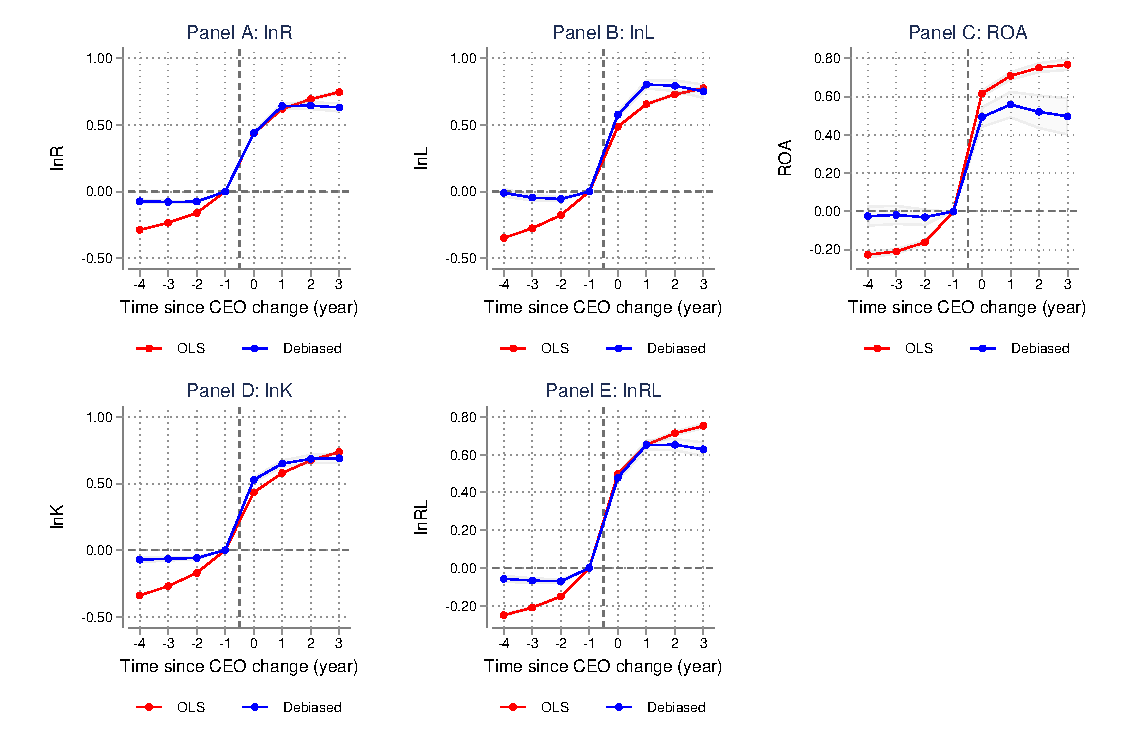
\includegraphics[width=17cm]{figure/outcomes_full.pdf}
\caption{Naive and Debiased Event-Time Estimates Around CEO Transitions}
\label{fig:dynamics}
\vspace{.2cm}

\begin{minipage}{15cm}
\footnotesize {Notes: Event-time dynamics of naive (red line) and placebo-controlled debiased (blue line) coefficients and 95\% confidence intervals. $\Delta z$ measured by $lnR$. $lnR$ = log revenue; $lnL$ = log labor; $lnK$ = log tangible assets; ROA = return on assets; $lnRL$ = log labor productivity.}
\end{minipage}
\end{figure}


\clearpage

\begin{table}[h]
    \centering
    \caption{Monte Carlo Parameters by Scenario}
    \vspace{.2cm}
    \label{tab:table_MC}
    & Baseline & Excess Variance & E. V. with Correction & Long Panel\\
\addlinespace$\hat Var(dz) (OLS) & $1.782^{}$ & $2.121^{}$ & $2.121^{}$ & $2.045^{}$ & \\
$\hat Var(dz)$ (debiased) & $1.003^{}$ & $1.343^{}$ & $1.343^{}$ & $1.019^{}$ & \\
\addlinespace$\hat Cov(dz, dy)$ (OLS) & $1.831^{}$ & $2.193^{}$ & $2.193^{}$ & $1.890^{}$ & \\
$\hat Cov(dz,dy)$ (debiased) & $0.996^{}$ & $1.365^{}$ & $1.191^{}$ & $1.013^{}$ & \\
\addlinespace $ R^2$ (Naive) & $0.808^{}$ & $0.779^{}$ & $0.779^{}$ & $0.643^{}$ & \\
$ R^2$ (debiased) & $0.608^{}$ & $0.622^{}$ & $0.520^{}$ & $0.578^{}$ & 
    \begin{minipage}{15.5cm}
    \vspace{.2cm}
    \footnotesize{Notes: Naive and placebo debiased coefficients and the values of the corresponding $R^2$ in Monte-Carlo simulations (50,000 treated firms and 50,000 control firms). Estimation of $\Delta z$ on lnR, when $\Delta z$ is measured by lnR. Treatment (placebo treatment) year drawn from a geometric distribution with a constant hazard of CEO change. Column 1 (baseline scenario): $\sigma(\Delta z) = 1$, $\sigma(\epsilon) = 0.71$, $\rho=0.9$, $T_1=T_2=4$; Column 2-3 (excess variance): $\sigma(\epsilon) = 1.2 \cdot 0.71$ in the treated group; Column 4 (long panel): firm spells are raised to $T_1=T_2=10$. $R^2$: the estimation based on all years (ATET); $R^2 \text{ at } t =3)$: the estimation is based on the difference between three years after relative to the year precedent to the treatment.}
    \end{minipage}
\end{table}
\vspace{.5cm}

\begin{table}
    \centering
    \caption{Characteristics of Firms With and Without a CEO Replacement}
    \vspace{.2cm}
    \label{tab:switch_desc}
    \begin{tabular}{lccccccc}
\hline\hline
 & lnR & Exporter & lnL & lnK & ROA & lnRL & N \\
\hline
Without CEO Switch & $10.0$ & $0.1$ & $1.4$ & $7.9$ & $2.5$ & $8.6$ & $220136$ \\
 & ($1.7$) & ($0.3$) & ($0.9$) & ($2.2$) & ($9.8$) & ($1.4$) &  \\
With CEO Switch & $10.2$ & $0.1$ & $1.5$ & $8.3$ & $2.2$ & $8.7$ & $231710$ \\
 & ($1.9$) & ($0.3$) & ($1.0$) & ($2.4$) & ($9.0$) & ($1.4$) &  \\
Growth & $-0.008$ & $-0.204$ & $-0.079$ & $-0.003$ & $-0.057$ & $0.004$ &  \\
 & ($0.185$) & ($0.760$) & ($0.657$) & ($0.284$) & ($374.204$) & ($0.192$) &  \\
Pre-trend & $0.004$ & $-0.154$ & $-0.007$ & $-0.003$ & $-0.080$ & $0.006$ &  \\
 & ($0.114$) & ($0.498$) & ($0.433$) & ($0.240$) & ($85.598$) & ($0.125$) &  \\
\hline\hline
\end{tabular}

    \begin{minipage}{16cm}
    \vspace{.2cm}
    \footnotesize{Notes: the first two lines of the table present the mean (standard deviation) firm characteristics with and without CEO replacement. The third and fourth lines show the proportional change of firm characteristics around and before CEO replacement. Around CEO replacement = $(\bar y_{after} - \bar y_{before})/\bar y_{before}$}, before CEO replacement = $(y_{-1} - y_{4})/y_{-4}$. 
    \end{minipage}
\end{table}
\vspace{.5cm}


\begin{table}
    \centering
    \caption{Analysis of Variance -- Naive and Debiased Estimates}
    \vspace{.2cm}
    \label{tab:table_application}
    \begin{tabular}{l*{5}{c}}
\hline\hline
 Estimate & lnR & lnL & lnK & ROA & lnRL \\
\hline
\addlinespace $ R^2$ (OLS) & $0.677$ & $0.672$ & $0.653$ & $0.642$ & $0.646$ \\
$ R^2$ (debiased) & $0.309$ & $0.256$ & $0.268$ & $0.185$ & $0.292$ \\
\hline\hline
\end{tabular}

    \begin{minipage}{9cm}
    \vspace{.2cm}
    \footnotesize{Notes: N = 2,551,515. The table presents the naive and placebo-controlled debiased estimated coefficients and the corresponding $R^2$ of CEO replacement. The variable used for estimating $\Delta z$ is log revenue (top panel), return on assets (bottom panel). lnR = log revenue; lnL = log labor; lnK = log tangible assets; ROA = return on assets; lnRL = log labor productivity.}
    \end{minipage}
\end{table}

\begin{table}
    \centering
    \caption{Analysis of Variance in Subsamples}
    \vspace{.2cm}
    \label{tab:table_heterogeneity}
    \begin{tabular}{l*{6}{c}}
\hline\hline
Samples & lnR & lnL & lnK & ROA & lnRL & N \\
\hline
One-to-One & $0.346$ & $0.284$ & $0.295$ & $0.197$ & $0.330$ & $1909382$ \\
Twos & $0.277$ & $0.241$ & $0.236$ & $0.188$ & $0.246$ & $2004282$ \\ \hline
Founder-to-Non & $0.390$ & $0.304$ & $0.328$ & $0.224$ & $0.382$ & $1162079$ \\
Non-to-Non & $0.328$ & $0.295$ & $0.307$ & $0.205$ & $0.315$ & $1631531$ \\ \hline
Gender switch & $0.334$ & $0.269$ & $0.277$ & $0.194$ & $0.308$ & $1913895$ \\
No gender switch & $0.297$ & $0.254$ & $0.269$ & $0.198$ & $0.283$ & $2002551$ \\ \hline
Age gap & $0.349$ & $0.288$ & $0.303$ & $0.198$ & $0.332$ & $1439578$ \\
No age gap & $0.335$ & $0.276$ & $0.270$ & $0.194$ & $0.317$ & $1047934$ \\ \hline
Max Emp. <10 & $0.311$ & $0.245$ & $0.270$ & $0.168$ & $0.298$ & $1260772$ \\
Max Emp. 11-50 & $0.315$ & $0.275$ & $0.263$ & $0.200$ & $0.269$ & $1003888$ \\
Max Emp. 51-100 & $0.308$ & $0.261$ & $0.245$ & $0.191$ & $0.205$ & $325426$ \\
Max Emp. 100+ & $0.348$ & $0.338$ & $0.278$ & $0.284$ & $0.250$ & $298148$ \\ \hline
Pre 2000 switch & $0.262$ & $0.240$ & $0.247$ & $0.147$ & $0.223$ & $521375$ \\
Post 2000 switch & $0.330$ & $0.266$ & $0.281$ & $0.207$ & $0.314$ & $2618528$ \\
\hline\hline
\end{tabular}

    \begin{minipage}{10cm}
    \vspace{.2cm}
    \footnotesize{The table presents the placebo-controlled debiased estimated $R^2$ of CEO replacement for various subsamples defined by CEO switch characteristics. lnR = log revenue.}
    \end{minipage}
\end{table}

\clearpage

%%%%%%%%%%%%%%%%%%%%%%%%%%%%%%%%%%%%%%%%%%%%%%
\section*{Appendix A: Derivation of Bias Terms}\label{sec: appA}
%%%%%%%%%%%%%%%%%%%%%%%%%%%%%%%%%%%%%%%%%%%%%%

\setcounter{equation}{0}
\renewcommand{\theequation}{A\arabic{equation}}

This appendix provides the formal matrix algebra derivation of the bias terms in second moments of estimated CEO effects.

\subsection{Matrix Notation Setup}

\paragraph{Model setup.} Let firm $i$ be observed for $T$ periods with outcome path $\mathbf y_i\in\mathbb R^T$ that decomposes into a (piecewise-constant) manager-effect path $\mathbf z_i$ and shocks $\mathbf e_i$. The model is
\begin{equation}
\mathbf y_i = \mathbf \alpha_i + \mathbf z_i + \mathbf e_i
\end{equation}
with 
\begin{equation}
\mathbb E[\mathbf z_i\mathbf z_i']= \mathbf \Lambda_i=
\begin{bmatrix}
  \lambda_{i11}\otimes \mathbf{11}' & \lambda_{i12}\otimes \mathbf{11}'\\
  \lambda_{i12}\otimes \mathbf{11}' & \lambda_{i22}\otimes \mathbf{11}'
\end{bmatrix},
\qquad \mathbb E[\mathbf z_i\mathbf e_i']=0,
\qquad \mathbb E[\mathbf e_i\mathbf e_i']=\sigma_1\mathbf\Sigma
\end{equation}
for changing firms, and 
\begin{equation}
\mathbb E[\mathbf z_i\mathbf z_i']= \mathbf \Lambda_i=
  \lambda_{i11}\otimes \mathbf{11}',
\qquad \mathbb E[\mathbf z_i\mathbf e_i']=0,
\qquad \mathbb E[\mathbf e_i\mathbf e_i']=\sigma_0\mathbf\Sigma
\end{equation}
for non-changing firms. The first equation is notation for the variance and covariance of manager fixed effects at firm $i$. The second equation states strict exogeneity (random mobility): every period's shock is mean independent of the entire CEO path. The third assumption allows for arbitrary autocorrelation in shocks over time but assumes that this autocorrelation is the same for changing and non-changing firms, up to a scalar multiplier $\sigma_1/\sigma_0$ (proportional autocovariance).

\paragraph{Projection Matrix and LSDV Estimator.} Define design matrix $\mathbf D$ and spell-length matrix $\mathbf T$. For $T_1=2$, $T_2=3$:
\[
  \mathbf D = \begin{bmatrix}
    1 & 0\\
    1 & 0\\
    0 & 1\\
    0 & 1\\
    0 & 1
  \end{bmatrix},
\]
and the diagonal matrix of spell lengths $\mathbf T$ as
$$
  \mathbf T = \operatorname{diag}(T_1,T_2)=\operatorname{diag}(2,3).
$$
The projection matrix that converts outcomes to within-spell means is
$$
  \mathbf P = \mathbf D\,\mathbf T^{-1}\,\mathbf D'.
$$
In the example,
\[
  \mathbf P = \begin{bmatrix}
    1/2 & 1/2 & 0 & 0 & 0\\
    1/2 & 1/2 & 0 & 0 & 0\\
    0 & 0 & 1/3 & 1/3 & 1/3\\
    0 & 0 & 1/3 & 1/3 & 1/3\\
    0 & 0 & 1/3 & 1/3 & 1/3
  \end{bmatrix}\quad\Rightarrow\quad
  \mathbf {Py}_i = 
  \mathbf\alpha_i +
  \begin{pmatrix}
  \frac12 \sum_{t=-2}^{-1} (z_{it} + e_{it}) \\
  \frac12 \sum_{t=-2}^{-1} (z_{it} + e_{it}) \\
  \frac13 \sum_{t=0}^{+2} (z_{it} + e_{it})\\
  \frac13 \sum_{t=0}^{+2} (z_{it} + e_{it})\\
  \frac13 \sum_{t=0}^{+2} (z_{it} + e_{it})
  \end{pmatrix}.
\]
Here $\mathbf P$ is idempotent, symmetric, and $\mathbf P\mathbf z_i = \mathbf z_i$.

The least-squares dummy variable (LSDV) estimator of the CEO effects is
\begin{equation}\label{eq:lsdv_appendix}
  \hat{\mathbf z}_i = \mathbf P\mathbf y_i - \hat{\mathbf \alpha}_i = \mathbf z_i + \mathbf P\mathbf e_i.
\end{equation}  
The estimated CEO effects are the true effects plus the within-spell mean of shocks. (For our method, it does not matter how firm fixed effects $\hat{\mathbf \alpha}_i$ are estimated, as we difference out firm means in all contrasts.)

\subsection{Population Moments and Bias Terms}

The relevant moments are
\begin{align}
  \mathbb E[\hat{\mathbf z_i}] &= \mathbf z_i,\\
  \mathbb E[\hat{\mathbf z_i}\hat{\mathbf z_i}'] &= 
\mathbb E[(\mathbf z_i + \mathbf P\mathbf e_i)(\mathbf z_i + \mathbf P\mathbf e_i)' ] =
    \mathbf \Lambda_i + \sigma\mathbf P\mathbf\Sigma\mathbf P,\\ 
  \mathbb E[\hat{\mathbf z_i}\mathbf e_i'] &= 
\mathbb E[(\mathbf z_i + \mathbf P\mathbf e_i)\mathbf e_i' ] = \sigma\mathbf P\mathbf\Sigma,\\
  \mathbb E[\hat{\mathbf z_i}\mathbf y_i'] &= 
\mathbb E[(\mathbf z_i + \mathbf P\mathbf e_i)(\mathbf z_i + \mathbf e_i)' ] = \mathbf \Lambda_i + \sigma\mathbf P\mathbf\Sigma.
\end{align}
These show variance inflation by $\sigma\mathbf P\mathbf\Sigma\mathbf P$ and contaminated covariances.

\subsection{Bias in Regression Slopes}

For any linear contrast with weights $\mathbf w\in\mathbb R^T$ and $\mathbf w'\mathbf 1=0$, define the estimated effect for the contrast by
$$
\Delta\hat z_i = \mathbf w'\hat{\mathbf z}_i = \mathbf w'\mathbf P\,\mathbf y_i = \Delta z_i + \eta_i,\qquad \eta_i:=\mathbf w'\mathbf P\,\mathbf e_i,
$$
and recall that $\Delta y_i = \Delta z_i + \varepsilon_i$ where $\varepsilon_i=\mathbf w'\mathbf e_i$. 

The naive regression slope is
\begin{equation}
\hat\beta = 
  \frac {\Cov(\Delta \hat z_i, \Delta y_i)}
        {\Var(\Delta \hat z_i)} =
  \frac {\mathbf w' \mathbb E[\hat{\mathbf z_i}\mathbf y_i ']\mathbf w}
        {\mathbf w' \mathbb E[\hat{\mathbf z_i}\hat{\mathbf z_i}']\mathbf w} =
  \frac {\mathbf w' [\mathbf \Lambda_i + \sigma \mathbf P\mathbf\Sigma]\mathbf w}
        {\mathbf w' [\mathbf \Lambda_i + \sigma \mathbf P\mathbf\Sigma\mathbf P]\mathbf w} =
  \frac {\lambda_i + \sigma \mathbf w' \mathbf P\mathbf\Sigma \mathbf w}
        {\lambda_i + \sigma \mathbf w' \mathbf P\mathbf\Sigma \mathbf P \mathbf w}. 
\end{equation}  

\textit{Covariance bias term.} $\Cov(\varepsilon_i,\eta_i)$ inflates the numerator when shocks are persistent and spells short.

\textit{Variance bias term.} $\Var(\eta_i)>0$ attenuates the denominator.

Both biases vanish as $T_1,T_2\to\infty$. 

\subsection{Sample Moments Across Heterogeneous Groups}

With $G$ groups of sizes $N_g$, sample moments are
\begin{align}
\widehat{\Cov}(\Delta y_i,\Delta \hat z_i) &= \sum_{g=1}^G \frac{N_g}{N} \widehat{\Cov}_g(\Delta y_i,\Delta \hat z_i)\\
\widehat{\Var}(\Delta \hat z_i) &= \sum_{g=1}^G \frac{N_g}{N} \widehat{\Var}_g(\Delta \hat z_i)
\end{align}

The expected values are
\begin{align}
\mathbb E\widehat{\Cov}(\Delta y_i,\Delta \hat z_i) &= \sum_{g=1}^G \frac{N_g}{N} \left[ 
\Bar\lambda_g
+ \sigma_g \mathbf w_g' \mathbf P_g\mathbf\Sigma \mathbf w_g\right] = 
\Bar\lambda +\sum_{g=1}^G \frac{N_g}{N} \sigma_g \mathbf w_g' \mathbf P_g\mathbf\Sigma \mathbf w_g\\
\mathbb E\widehat{\Var}(\Delta \hat z_i) &= \sum_{g=1}^G \frac{N_g}{N} \left[ 
\Bar\lambda_g
+ \sigma_g \mathbf w_g' \mathbf P_g\mathbf\Sigma \mathbf P_g \mathbf w_g\right] = 
\Bar\lambda +\sum_{g=1}^G \frac{N_g}{N} \sigma_g \mathbf w_g' \mathbf P_g\mathbf\Sigma \mathbf P_g \mathbf w_g
\end{align}

Here $\Bar\lambda$ is the average CEO effect variance. Bias terms depend on $\mathbf P_g$, $\mathbf w_g$, and $\sigma_g\mathbf\Sigma$, making direct estimation impractical with complex $\mathbf\Sigma$.

\clearpage

%%%%%%%%%%%%%%%%%%%%%%%%%%%%%%%%%%%%%%%%%%%%%%%%%%%%
\section*{Appendix B: Additional Figures and Tables}
%%%%%%%%%%%%%%%%%%%%%%%%%%%%%%%%%%%%%%%%%%%%%%%%%%%%

\renewcommand{\thefigure}{B\arabic{figure}} 
\renewcommand{\thetable}{B\arabic{table}}
\setcounter{figure}{0}
\setcounter{table}{0}


\begin{table}[h]
    \centering
    \caption{Company-Year Characteristics}
    \vspace{.2cm}
    \label{tab:year_desc}
    \begin{tabular}{l*{3}{c}}
\hline\hline
Year & Frims & CEO Switches & Employment \\
\hline
1995  & 76866 & 3921 & 13 \\
2000  & 133686 & 10043 & 10 \\
2005  & 145956 & 8772 & 9 \\
2010  & 138815 & 8684 & 9 \\
2015  & 158242 & 10733 & 9 \\
2020  & 174683 & 10714 & 9 \\
Total  & 4107611 & 262973 & 10 \\
\hline\hline
\end{tabular}

    \begin{minipage}{8.5cm}
    \vspace{.2cm}
    \footnotesize{Notes: the table presents the number of firms, number of CEO replacements, and average employment of firms in the data in various years.}
    \end{minipage}
\end{table}
\vspace{.5cm}


\begin{table}[h]
    \centering
    \caption{Industrial Distribution of Firms}
    \vspace{.2cm}
    \label{tab:industry_desc}
    \begin{tabular}{l*{2}{c}}
\hline\hline
Industry & N & \% \\
\hline
Agriculture & $141867$ & $3.5$ \\
Industry & $578437$ & $14.1$ \\
Construction & $447245$ & $10.9$ \\
Trade & $1122181$ & $27.3$ \\
Business Services & $662333$ & $16.1$ \\
Other Services & $1155548$ & $28.1$ \\
\hline\hline
\end{tabular}

    \begin{minipage}{10cm}
    \vspace{.2cm}
    \footnotesize{\hspace{1.8cm} Notes: Distribution of firms by sector.}
    \end{minipage}
\end{table}
\vspace{.5cm}


\begin{table}[h]
    \centering
    \caption{CEO Tenure}
    \vspace{.2cm}
    \label{tab:tenure_desc}
    \begin{tabular}{lcccc}
    \begin{tabular}{l*{3}{c}}
\hline\hline
Statistic & P25 & P50 & P75 \\
\hline
Firm max age & $.$ & $.$ & $.$ \\
1st CEO tenure & $2.00$ & $5.00$ & $10.00$ \\
2nd CEO tenure & $2.00$ & $4.00$ & $8.00$ \\
3rd CEO tenure & $2.00$ & $4.00$ & $7.00$ \\
4th or higher CEO tenure & $2.00$ & $3.00$ & $6.00$ \\
% of firms with 2 CEOs & $0.28$ & $.$ & $.$ \\
% of firms with CEO switches & $0.48$ & $.$ & $.$ \\
Nr. of Firms & $537998.00$ & $.$ & $.$ \\
\hline\hline
\end{tabular}

    \end{tabular}
    \begin{minipage}{8cm}
    \vspace{.2cm}
    \footnotesize{Notes: distribution of the length of tenure of CEOs. Tenure measured in years.}
    \end{minipage}
\end{table}
\vspace{.5cm}

\end{document}